\documentclass[oneside,final,14pt,a4paper]{extreport}

\usepackage{algorithm}
\usepackage{algpseudocode}

\usepackage{tempora} % Times New Roman alike font
\usepackage[color={red!100!green!33},textwidth=3cm,obeyFinal]{todonotes}

\usepackage{vmargin}
\setpapersize{A4}
\setmarginsrb{2.5cm}{2.2cm}{2.2cm}{2.2cm}{0pt}{10mm}{0pt}{13mm}
\usepackage{setspace}
\setstretch{1.5}
\usepackage{indentfirst}
\parindent=1.25cm

%%%%% ADDED TO SUPPORT TT BOLD FACES %%%%
\DeclareFontShape{OT1}{cmtt}{bx}{n}{<5><6><7><8><9><10><10.95><12><14.4><17.28><20.74><24.88>cmttb10}{}
\renewcommand{\ttdefault}{pcr}
%%%%% END %%%%%%%%%%%%%%%%%%%%%%%%%%%%%%% 

\usepackage{atbegshi,picture}
%\usepackage[T1,T2A]{fontenc}
%\usepackage[utf8]{inputenc}

\usepackage[english]{babel}
\usepackage[backend=biber,style=ieee,autocite=inline]{biblatex}
\bibliography{ref.bib}
\DefineBibliographyStrings{english}{%
  bibliography = {References},}
\usepackage{blindtext}

\usepackage{pdfpages}
\newenvironment{bottompar}{\par\vspace*{\fill}}{\clearpage}
\usepackage{amsmath,amssymb,  amsfonts}
\usepackage{url}
\usepackage{amsthm}
\newtheorem{theorem}{Theorem}
\newtheorem{corollary}{Corollary}
\newtheorem{lemma}{Lemma}
\newtheorem{proposition}{Proposition}
\theoremstyle{definition}
\newtheorem{definition}{Definition}
\theoremstyle{remark}
\newtheorem*{remark}{Remark}
\theoremstyle{remark}
\newtheorem*{example}{Example}

\usepackage{float}
\usepackage{graphicx}
\graphicspath{{figs/}} %path to images
\usepackage{array}
\usepackage{multirow,array}
\usepackage{caption}
\usepackage{subcaption}
\usepackage{hyperref}
\hypersetup{colorlinks=true, linkcolor=black, citecolor=black}
\usepackage{paralist}
\usepackage{listings, listings-rust}
% kolayne: Inclusion of zed-csp breaks pseudocode algorithms
%\usepackage{zed-csp}
\usepackage{fancyhdr}
\usepackage{csquotes}
\usepackage{color}
% \usepackage{anyfontsize}
% \usepackage{mathptmx}
% \usepackage{t1enc}

\usepackage{chngcntr}
\usepackage{upgreek} 
\usepackage{bm}
\usepackage{hyperref}
\usepackage{booktabs}
\usepackage{multirow}
\usepackage{longtable}
\usepackage[font=singlespacing, labelfont=bf]{caption}
%Hints
\newcommand\pic[1]{(Fig. \ref{#1})} %Ref on figure
\newcommand\tab[1]{(Tab. \ref{#1})} %Ref on table

\setlength{\headheight}{32.0976pt}
\usepackage[shortlabels]{enumitem}
\newlist{inlinelist}{enumerate*}{1}
\setlist*[inlinelist,1]{%
  label=(\arabic*),
}

% \setcounter{secnumdepth}{4}
\captionsetup[table]{labelfont={normalfont}, name={TABLE}, labelsep={newline}}
\setlength{\parindent}{2em} 
\DeclareCaptionLabelSeparator{figSep}{.\quad}
\captionsetup[figure]{labelfont={normalfont}, name={Fig.}, labelsep=period}
\counterwithin{figure}{chapter}

% \usepackage{titlesec}
% \titleformat{\section}[hang]{\fontsize{20}{24}\selectfont\filcenter}{\Roman{section}}{1em}{}
% \titleformat{\subsection}[hang]{\itshape}{\Alph{subsection}.}{1em}{}[]
% \titleformat{\subsubsection}[runin]{\itshape}{\arabic{subsubsection})}{1em}{}[$:$]
% \titlespacing{\subsubsection}{1em}{1em}{1em}
% \titleformat{\paragraph}[runin]{\itshape}{\alph{paragraph})}{1em}{}[$:$\quad]
% \titlespacing{\paragraph}{2em}{1em}{1em}

\usepackage{placeins} % for \FloatBarrier

\pagestyle{fancyplain}

% remember section title
\renewcommand{\chaptermark}[1]%
	{\markboth{\chaptername~\thechapter~--~#1}{}}

% subsection number and title
\renewcommand{\sectionmark}[1]%
	{\markright{\thesection\ #1}}

\rhead[\fancyplain{}{\bf\leftmark}]%
      {\fancyplain{}{\bf\thepage}}
\lhead[\fancyplain{}{\bf\thepage}]%
      {\fancyplain{}{\bf\rightmark}}
\cfoot{} %bfseries


\newcommand{\dedication}[1]
   {\thispagestyle{empty}
     
   \begin{flushleft}\raggedleft #1\end{flushleft}
}

\if@todonotes@disabled
\newcommand{\hlfix}[2]{#1}
\else
\newcommand{\hlfix}[2]{\hl{#1}\todo{#2}}
\fi

\lstloadlanguages{Rust}
\lstset{language=Rust, style=colouredRust}

\begin{document}

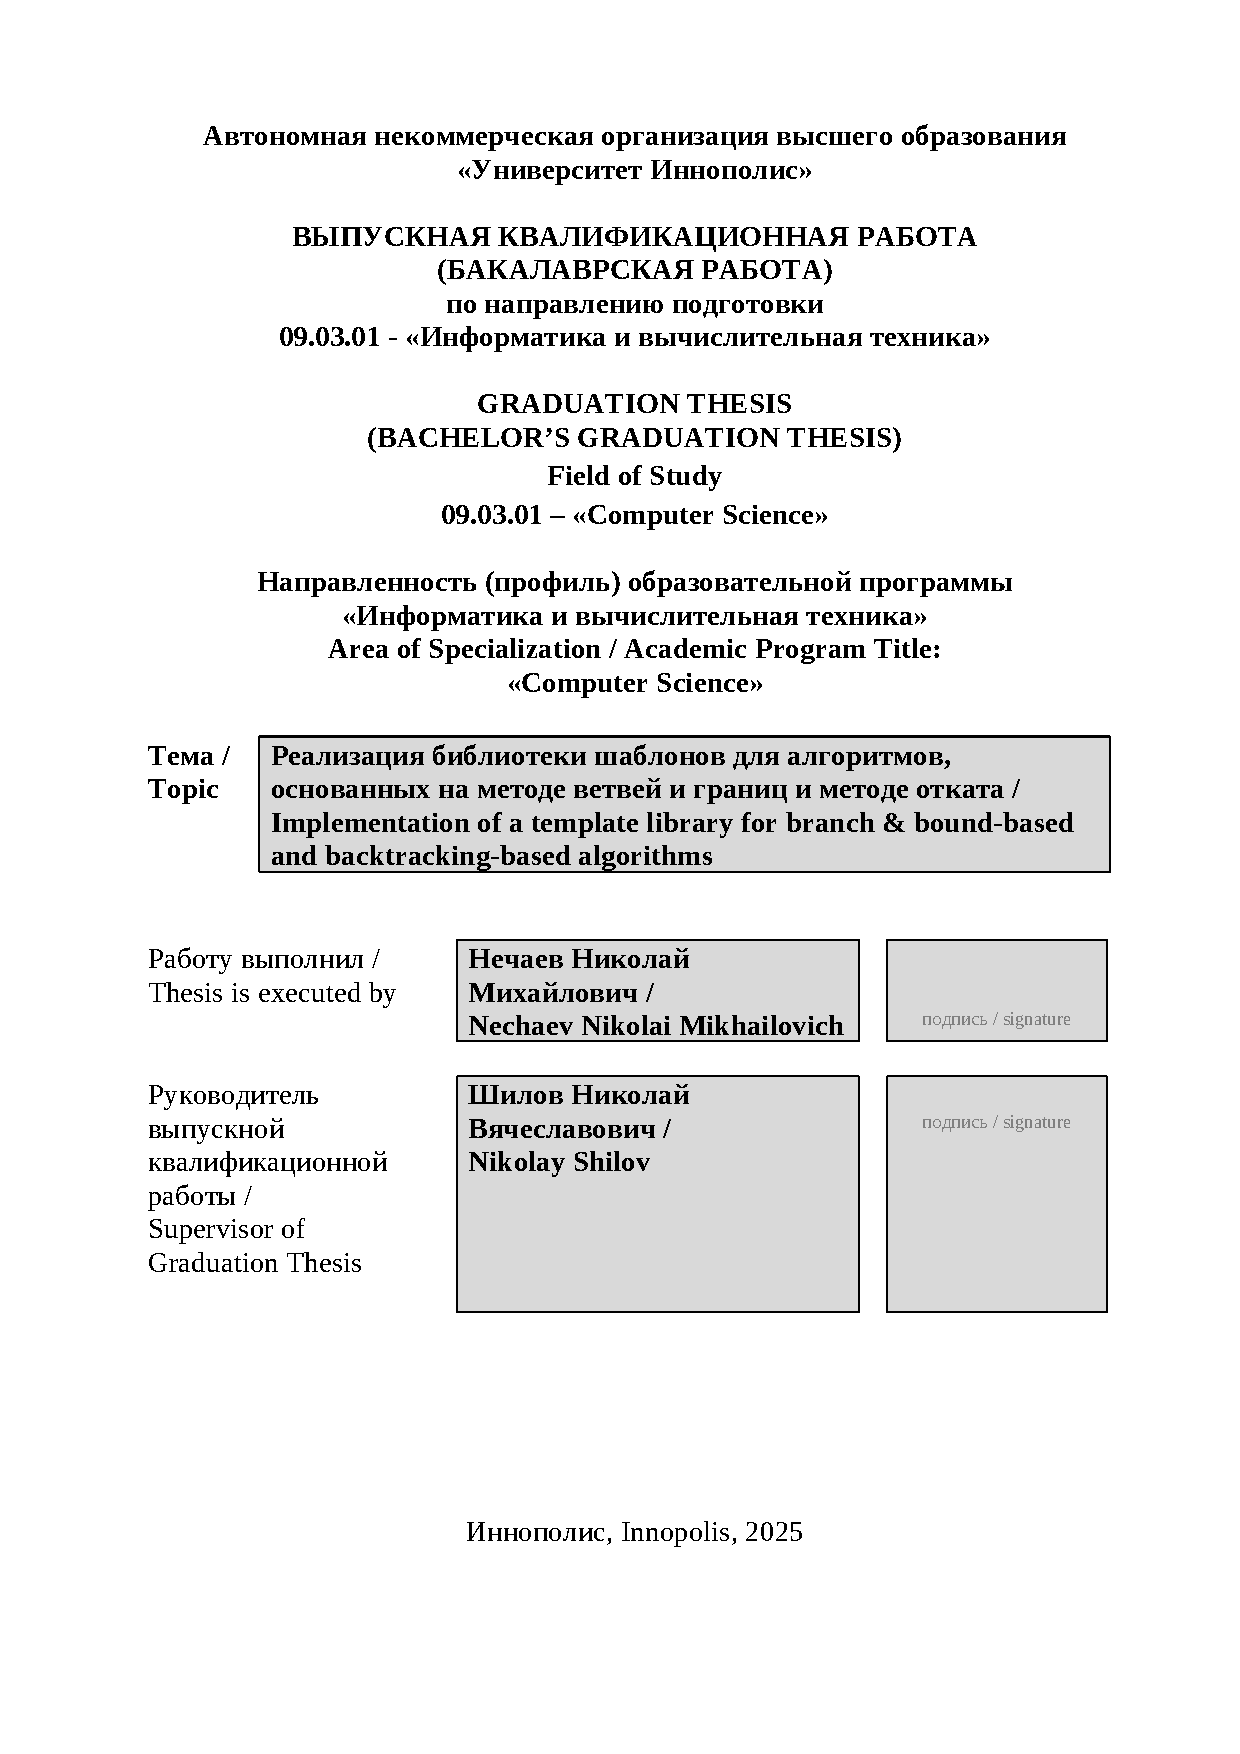
\includepdf[pages=-,offset=75 -80]{title.pdf}
\tableofcontents
\lstlistoflistings
\listoftables
%\listoffigures
\newpage


\begin{abstract}
% skip one line to make the abstract start with indent

\end{abstract}

\setcounter{page}{8}
% set manually the number, from which Chapter 1 starts!
% Why do we put 7 in this case?
% Title page - page 1
% Contents - page 2, page 3, page 4
% List of tables - page 5
% List of figures - page 6
% List of listings - page 7
% Abstract - page 8
% Chapter 1 - page 9
% In your thesis the counter number can be different, please count carefully and insert the corresponding number.

\chapter{Introduction}
\label{chap:intro}

This chapter aims to give an intuitive understanding of the branch-and-bound and
the backtracking methods, provide examples of problems commonly solved with these methods,
and present the goal of the presented work.

\section{Backtracking and branch-and-bound methods}

Backtracking and branch-and-bound (B\&B) methods are methods used in
algorithms for solving discrete optimization problems. Both methods are also used for solving
% TODO: IS THERE A TERM FOR SUCH PROBLEMS??
algorithmic problems where it is sufficient to find a single solution under given constraints
(e.g., Sudoku) -- such problems can be seen as special cases of discrete optimization with
trivial objective functions.

Both methods solve a problem by splitting it into subproblems recursively until reaching a
subproblem that is trivial enough to be solved directly. During this process, generated
subproblems are evaluated, taking into account the current best solution
candidate (\emph{incumbent}): if it can be determined that the best potentially
achievable solution to a subproblem is not better than the incumbent, that subproblem is
rejected, and its subproblems are not considered.

% TODO: IS THERE A TERM FOR SUCH PROBLEMS?? (I called them `single-solution` here)
In the special case of a single-solution problem (such as Sudoku), no candidate solution
is better than any other candidate solution, thus, as soon as any solution is found,
all other subproblems can be rejected, and the algorithm can terminate.

The primary difference between the backtracking and branch-and-bound methods
is in the order in which subproblems are generated and evaluated. A backtracking-based
algorithm, given a problem, will first generate and fully evaluate the first subproblem
of the given problem, and process all of its subproblems until all the candidate solutions
are found or all the remaining subproblems are rejected; only after that will it proceed with
the second (and further) subproblem(s) of the given problem. Overall, this process is similar to
a depth-first search in a graph. In turn, a branch-and-bound-based algorithm, given a problem,
will generate all of its subproblems and add them to the set of subproblems to be considered
(\emph{live nodes}). On every iteration, the algorithm will select a subproblem from the set,
following some rule (e.g., first-come-first-served). Overall, this is similar to a breadth-first
search in a graph, although other selection rules or additional heuristics can be applied to
improve performance.

\section{Problem examples}

\subsection{Boolean satisfiability problem (CNF SAT)}

The Boolean satisfiability problem, sometimes abbreviated as CNF SAT, is as follows:
given a Boolean formula in the conjunctive normal form, find the set of variable assignments
for which the formula is satisfied (i.e., evaluates to true), if there is any.

For example, for the formula $a \land \neg b$, the assignment $a=\text{T}, b=\text{F}$
satisfies the formula; while the formula $a \land \neg a$ is \emph{unsatisfiable}.

The boolean satisfiability problem can be solved, e.g., with the following backtracking-based
algorithm: a recursive function accepts a formula, the current variable assignment
(initially, an empty set), and a queue of variables left to assign. The function pops a
variable from the queue and gets a variable to assign a value to. For every possible variable
value (namely, true and false), the function tries to assign it to the variable
and solve the problem recursively. If the solution is not found, another assignment is
attempted. The first solution found is returned.

Here is a pseudo-code implementation of the function:

\begin{algorithm}
\begin{algorithmic}
\Procedure{solve}{formula, assignment, varsLeft}
    \If {$varsLeft = \varnothing$}
        \State \Return{$assignment$}
    \EndIf

    \State

    \State $nextVar \gets varsLeft.pop()$
    \ForAll{$val \in \{\text{T}, \text{F}\}$}
        \State $assignment \gets assign(assignment, nextVar, val)$
        \If{$\neg unsatisfied(formula, assignment)$}
            \State $solution \gets solve(formula, assignment, varsLeft)$
            \If{$solution \neq \varnothing$}
                \State \Return{$solution$}
            \EndIf
        \EndIf
    \EndFor

    \State

    \State \Return{$\varnothing$}
\EndProcedure
\end{algorithmic}
\end{algorithm}

where $assign(assignment, var, val)$ returns the updated assignment by setting the value
of variable $var$ to $val$; $unsatisfied(formula, assignment)$ evaluates the formula and
returns true if the formula is already known to be unsatisfied, given the variable assignment.

\subsection{Knapsack problem}

The Knapsack problem is as follows: given a lifting capacity value and a set of items,
each having a weight and a price, find a subset of items that has the maximum possible
cumulative price given that cumulative weight shall not exceed the lifting capacity value.

The Knapsack problem can be solved, e.g., with the following branch-and-bound-based algorithm:
a function maintains the current best solution (initially, an empty knapsack) and a queue where
each entry represents a pre-packed Knapsack and is a triple of:
price accumulated, lifting capacity left, set of unprocessed items. On every iteration,
an entry is popped from the queue and evaluated: if it has a potential of surpassing the
current best solution (see below for details), an item is extracted from the set of unprocessed items, and two options are considered: including the item (if possible) and not including it.
The corresponding entries are added to the queue.

Here is a pseudo-code implementation of the function:

\begin{algorithm}
\begin{algorithmic}
\Procedure{solve}{items, maxWeight}
    \State $queue \gets \{(0, maxWeight, items)\}$
    \State $incumbentPrice \gets 0$
    \State $incumbent \gets \varnothing$
    \While{$queue \neq \varnothing$}
        \State $entry \gets queue.pop()$
        \If{$maxAchievablePrice(entry) > incumbentPrice$}
            \State $(price, capacity, items) \gets entry$
            \State $(iPrice, iWeight) \gets items.pop()$
            \If{$capacity \ge iWeight$}
                \State $queue.push((price + iPrice, capacity - iWeight, items))$
            \EndIf
            \State $queue.push((price, capacity, items))$
        \EndIf
    \EndWhile
    \State \Return{$incumbent$}
\EndProcedure
\end{algorithmic}
\end{algorithm}

where $maxAchievablePrice$ is a function of entry that gives an upper boundary of the maximum
price achievable from the given state. One way to implement it (the one that was implemented
as part of the presented work) is to try to greedily include all remaining items starting with
the
most valuable ones, until the lifting capacity value is \emph{exceeded} (i.e., the constraint
is no longer satisfied). It can be shown that the cumulative price achieved in this case is
an upper boundary of the best value that can be achieved while satisfying the constraint.

\section{Goal of study}

The goal of the presented work is to design and develop a template library for implementing
backtracking- and B\&B-based algorithms without having to reimplement their common parts.

% =========== TEMPLATE STUFF BELOW ===========

%\chaptermark{Optional running chapter heading}
%\section{Spacing \& Type}
%\label{sec:section}

%This is a section. This is a citation without brackets. and this is one with brackets \cite{A}. Multiple \cite{A,B,C} Here's a reference to a subsection: \ref{sec:subsection}. Citation of an online article \cite{D}. Citation of an online proceeding \cite{F}. The body of the text and abstract must be double-spaced except for footnotes or long quotations. Fonts such as Times Roman, Bookman, New Century Schoolbook, Garamond, Palatine, and Courier are acceptable and commonly found on most computers. The same type must be used throughout the body of the text. The font size must be 10 point or larger and footnotes\footnote{This is a footnote.} must be two sizes smaller than the text\footnote{This is another footnote.} but no smaller than eight points. Chapter, section, or other headings should be of a consistent font and size throughout the ETD, as should labels for illustrations, charts, and figures.

%\subsection{Creating a Subsection}
%\label{sec:subsection}

%\subsubsection{Creating a Subsubsection}
%\subsubsection{Creating a Subsubsection}
%\subsubsection{Creating a Subsubsection}

%\paragraph{This is a heading level below subsubsection}

%And this is a quote:
%
%\begin{quote}
%\blindtext
%\end{quote}

% \begin{figure}[hbt]
% \centering
% 
\includegraphics[]{figs/IU.png}
% \caption{One kernel at $x_s$ (\emph{dotted kernel}) or two kernels at
% $x_i$ and $x_j$ (\textit{left and right}) lead to the same summed estimate
% at $x_s$. This shows a figure consisting of different types of
% lines. Elements of the figure described in the caption should be set in
% italics, in parentheses, as shown in this sample caption.}
% \label{fig:example}
% \end{figure}
%
% This is a table:
% % currsize is not set in the long table environment, so we need to set it before we set it up.
% \makeatletter
% \let\@currsize\normalsize
% \makeatother
%
% % tabular environments are set to be single-spaced in the  thesis class,  but long tables do not use tabular
% % to get around this, set the spacing to single spacing at the start of the long table environment, and set it back to double-spacing at the end of it
%
% \begin{longtable}{c|c|c}
% \caption[This is the title I want to appear in the List of Tables]{This Is a Table Example} \label{tab:pfams} \\
% \hline
% A & B & C \\
% \hline
% \endfirsthead
% \multicolumn{3}{@{}l}{} \\
% \hline
% A & B & C\\
% \hline
% \endhead
% a1 & b1 & c1 \\
% a2 & b2 & c2\\
% a3 & b3 & c3\\
% a4 & b4 & c4\\
% \hline
% \end{longtable}
%
% The package ``upgreek'' allows us to use non-italicized lower-case greek letters. See for yourself: $\upbeta$, $\bm\upbeta$, $\beta$, $\bm\beta$. Next is a numbered equation:
% \begin{align}
% \label{eq:name}
% \|\bm{X}\|_{2,1}={\underbrace{\sum_{j=1}^nf_j(\bm{X})}_{\text{convex}}}=\sum_{j=1}^n\|\bm{X}_{.,j}\|_2
% \end{align}
% The reference to equation (\ref{eq:name}) is clickable.
% \section[Theorems, Corollaries, Lemmas, Proofs, Remarks, Definitions and Examples]{Theorems, Corollaries, Lemmas, Proofs, Remarks, Definitions,and Examples}
%
% \begin{theorem}
% \label{thm:onlytheorem}
% \blindtext
% \end{theorem}
%
% \begin{proof}
% I'm a (very short) proof.
% \end{proof}
%
% \begin{lemma}
% I'm a lemma.
% \end{lemma}
%
% \begin{corollary}
% I include a reference to Thm. \ref{thm:onlytheorem}.
% \end{corollary}
%
% \begin{proposition}
% I'm a proposition.
% \end{proposition}
%
% \begin{remark}
% I'm a remark.
% \end{remark}
%
% \begin{definition}
% I'm a definition. I'm a definition. I'm a definition. I'm a definition. I'm a definition. I'm a definition. I'm a definition. I'm a definition. I'm a definition. I'm a definition. I'm a definition.
% \end{definition}
%
% \begin{example}
% I'm an example.
% \end{example}
%
%
% \section[Optional table of contents heading]{Section with\\ linebreaks in\\the
% name}
%
%
% \Blindtext[2]

\chapter{Literature Review}
\label{chap:lr}

\section{Questions}

Based on the goal, I formulated the following questions for the literature review. Because one
of the potential application areas suggested by my supervisor is reliable computing, one of
the questions relates to formalized branch-and-bound and backtracking methods.

LRQ\#1: What does the scientific community understand by branch-and-bound and backtracking methods?
What are the parts common to all branch-and-bound-based and backtracking-based algorithms?
Which parts of the the algorithms vary from problem to problem? \\

LRQ\#2: What were the previous attempts to formalize branch-and-bound and backtracking methods
and algorithms based on them? \\

LRQ\#3: What are ways in which these algorithms can be or are commonly implemented? \\

\section{Searching procedure}

For each question, I searched for articles in ScienceDirect,
Google Scholar, and ResearchGate, combining the following keywords to form search queries
for my questions:

\begin{itemize}
    \item Backtracking (method)
    \item Branch and bound (method)
    \item General / Generic
    \item Formal / Formalization / Verification (LRQ\#2)
\end{itemize}

\section{Answers to the questions}

\subsection{LRQ\#1: Understanding backtracking and branch-and-bound}

\subsubsection{Branch \& Bound method}

In the most general case studied in \cite{clausen1999principles}, \textbf{Branch \& Bound (B\&B)}
algorithms solve optimization problems, that is, minimize an \emph{objective function} in the
\emph{feasible solution space}, which is limited by constraints. To do this, B\&B algorithms
implement a search of a "dynamically developed" (lazily-generated) graph
(also referred to as \emph{virtual graph}
    \cite{shilov2011rutemplateverif, shilov2012verifmono}),
which acts as a search tree, where every node represents a subproblem derived from the
original problem through addition of constraints.

Initially, the tree consists of just the root node, which represents the original problem.
On every iteration, a node is extracted from the set of \emph{live nodes}.
It is then evaluated: the subproblem is broken down to
two \cite{narkawicz2013formalnasa} or more \cite{clausen1999principles}
subproblems according to a
\emph{branching rule}, new nodes become children of the evaluated node and are added
to the set of live nodes. The \emph{bounding function} is evaluated for nodes in
consideration: if the value of the bounding function at the candidate node is
not better than the value of the objective function at the current
best solution (\emph{incumbent}), the candidate can be discarded without descending into
its subtree, as its solution space cannot contain a solution better than the incumbent
(due to properties of the bounding function discussed below).

When a subproblem is trivial enough to be solved without branching, it is solved
and the objective function is evaluated at. The objective function values of the new
solution and the incumbent are compared, and the best one becomes the new incumbent.

\subsubsection{Problem-specific parts of B\&B}

While the core part of walking the search tree is common to all the B\&B algorithms,
there are parts that depend on a concrete problem that an algorithm is solving. They
are discussed below. For clarity, examples of the problem-specific parts are given
as in a Sudoku solving B\&B-based algorithm \cite{indriyono2024sudoku}. Every node
of the solution tree represents a partially filled Sudoku board.

The following problem-specific parts were identified \cite{clausen1999principles}:

\begin{itemize}
    \item \emph{Objective function} is a function of a feasible solution that the algorithm
        shall minimize.
        Objective function can be evaluated for a concrete solution
        (corresponding to a leaf node in the tree) rather than a solution space. \\
        As in Sudoku there is no "worse" or "better" solutions, only valid or invalid ones,
        a binary objective function could be defined, e.g., equal to
        $1$ for a valid solution and $2$ for an invalid solution (as less is better).

    \item \emph{Root node} represents the original problem to be solved. \\
        In the Sudoku example,
        the root node represents the pre-filled Sudoku board, as given initially;
        pre-filled values are the initial constraints.

    \item \emph{Branching rule} is an algorithm that breaks a problem down to subproblems
        (i.e., generates descendants of a node). \\
        The following shall hold for a branching rule to be valid:
        \begin{enumerate}[(a)]
        \item solution space of the parent node shall be equal to the union of solution spaces of its
            direct descendants, and
        \item solution spaces of sibling nodes shall not intersect (i.e.,
            constraints imposed on different descendants shall be mutually exclusive).
        \end{enumerate}

        In the Sudoku example, one option for a branching rule is to select an empty cell
        and try to insert every possible digit (1-9) in it, thus creating 9 descendants of a node.
        If the Sudoku board in a node does not have any empty cells, no further branching is possible,
        and that node is a leaf node.

    \item \emph{Bounding function} is a computationally cheap function of a solution subspace
        that estimates the best potentially achievable solution in that subspace.
        It can be evaluated for any subproblem. \\
        The following shall hold for a bounding function $g$ to be valid:
        \begin{enumerate}[(a)]
            \item Bounding function is no worse than the objective function $f$:
                \[
                g(\{X\}) \leq f(X) \:\text{for any feasible solution}\: X
                \]
            \item Narrowing solution space down shall not improve the best solution estimate:
                \[
                g(S) \leq g(S') \:\text{for}\: S \supseteq S'
                \]
                or, equivalently
                \[
                \forall S, T: g(S \cup T) \leq \min(g(S), g(T))
                \]
        \end{enumerate}

        In the Sudoku example, the bounding function will be used only to discard subtrees
        in which we can never find a solution (i.e., rule out partial solutions where the
        pre-filled part is already invalid). Thus, we could define
        the bounding function to be equal to $1$ if the partially filled board is valid and $2$
        otherwise.

        In the Sudoku example, the bounding function happens to be very similar to the objective
        function; in more advanced optimization problems, a more sophisticated bounding
        function would be useful.

    \item \emph{Selection strategy} is a strategy according to which a live node is selected
        at the beginning of every iteration. \\
        Common selection strategies are:
        \begin{itemize}
            \item Breadth-first search (BFS) evaluates nodes of the tree layer by layer;
            \item Best-first search (BeFS) greedily selects a node with the lowest value of the
                bounding function out of the live nodes; in the presented work this method
                is referred to as \emph{Greedy} search;
            \item Depth-first search (DFS) evaluates nodes in an order analogous to a
                depth-first search of a graph.
        \end{itemize}

        For some optimization problems, it makes sense to use BeFS to arrive at the first
        candidate solution earlier, thus discarding more solution spaces without
        descending into them.
        For the Sudoku example, however, it would not benefit the performance, as the bounding
        function conveys too little information about the solution subspace.
        In the example, it would be more effective to use DFS, which can be implemented
        with a more efficient data structure.

    \item \emph{Evaluation strategy}, either \emph{eager} or \emph{lazy}, determines when the
        algorithm compares candidate nodes against the incumbent to potentially discard them:
        \begin{itemize}
            \item With \emph{eager} evaluation, a selected live node is first \emph{branched}
                (i.e., split into subproblems), then
                new nodes are compared against the incumbent and are only inserted into the set
                of live nodes if they have the potential to produce a better solution
                (discarded otherwise);
            \item With \emph{lazy} evaluation, a node selected from the set of live nodes is first compared
                with the incumbent (and can be discarded at this point), then branched,
                and the descendant nodes are inserted to the set of live nodes unconditionally.
                \todo{(Nechaev) but what if we combine eager+lazy into an "aggressive" strategy:
                    evaluate both on insert and on extraction? - (Shilov) It makes sense, of course, but should be named "joint" rather than "aggressive".}
        \end{itemize}
\end{itemize}

\subsubsection{Backtracking and other special cases}

According to \cite{shilov2012verifmono, indriyono2024sudoku}, \textbf{backtracking}
is a method to solve optimization problem in a way similar to the one described above, except
that a depth-first search is used. So, it can be seen as a special case of branch-and-bound
with the specific subproblem consideration order. Although the term \emph{backtracking} is
sometimes used to refer to any kind of branch-and-bound \cite{finkel1987distrib},
in the presented work, \emph{backtracking} refers to a kind of branch-and-bound with the
depth-first tree traversal.

Brute-force search for optimization problems could be seen as another special case of the
Branch \& Bound method with the bounding function $g(x) = -\infty$.
Indeed, in this case, all nodes are evaluated
and no subtree is ever discarded, leading to the exhaustive search through all the possible solutions.

\subsection{LRQ\#2: What were the previous attempts to formalize branch-and-bound and backtracking methods and algorithms based on them?}

In \cite{narkawicz2013formalnasa}, authors present and formally verify a "generic branching
algorithm\footnote{The terms \emph{generic algorithm} and \emph{template} are used interchangeably
                    here and after}
for solving global optimization problems". Their algorithm template is to be instantiated with
functions (such as the objective function, the bounding function, etc) to form a concrete
algorithm for solving a concrete optimization problem, which would be easier to formally verify
because the core (generic) part of it is proven correct as long as supplied functions
satisfy certain criteria.

However, because the template in \cite{narkawicz2013formalnasa} was designed specifically for
numerical optimization problems, it does not fit the most general B\&B use case for the following
reasons:

\begin{enumerate}
    \item Because the researchers' goal was to simplify the verification of algorithms instantiated
        from their template, the template is specialized for numerical optimization. It moves the
        burden of verifying common numerical-related statements to the authors of the generic
        part of the algorithm, however, it makes it harder to use their template for other kinds of
        optimization problems. For example, the template in \cite{narkawicz2013formalnasa}
        is designed to branch in a way that only makes sense when the objective function is seen as
        a numerical function of multiple variables, each having a 1-dimensional domain.
    \item Some aspects of the branch-and-bound technique, such as evaluation strategy
        and selection strategy, can not be specialized in the
        generic algorithm from \cite{narkawicz2013formalnasa} because they are hard-coded into it.
\end{enumerate}

The work in \cite{narkawicz2013formalnasa} further continues in \cite{smith2015rigorous},
and is implemented as a C++ library called
Kodiak \footnote{Electronically available at \url{https://github.com/nasa/Kodiak}},
which was not itself formally verified, but, according to the authors, "closely follows
the formally verified depth-first branch and bound algorithm with generic types for problem domains
and solution types" (referring to \cite{narkawicz2013formalnasa}). Being an implementation of the
generic algorithm discussed above, it suffers from the same issues: it is specialized to solve
numerical optimization problems and does not allow to customize some aspects, such as the
virtual graph walk order.

\subsection{LRQ\#3: What are ways in which these algorithms can be or are commonly implemented?}

Both backtracking-based and branch-and-bound-based algorithms were previously implemented
for specific problems
(e.g., \cite{bard1990bilevel, breuel2003geometric, lalami2012gpu}),
as well as for generic cases with varying genericness
(e.g., \cite{narkawicz2013formalnasa, voloshinov2017implementation,
finkel1987distrib, prenner1972proglangs, johnson1988modular}).

In most cases, backtracking is implemented with recursive function calls,
e.g., in \cite{narkawicz2013formalnasa, bard1990bilevel},
and branch-and-bound is implemented with a queue or a priority queue,
depending on the selection strategy, e.g., in \cite{breuel2003geometric}.

In special cases, other technical implementations are used, although the computation logic
is generally the same. For example, in \cite{lalami2012gpu}, authors implement a
breadth-first search with items "sorted according to decreasing profit per weight ratio",
however, because in this work computations are parallelized with a GPU
(with some parts performed on a CPU), the technical implementation is somewhat more
sophisticated than a loop on a priority queue.

Distributed branch-and-bound search is another example in which the technical implementation
becomes more complicated, although it follows the same general model. For example,
in \cite{voloshinov2017implementation}, worker machines are assigned subtrees of the main search tree;
during the computation, they only exchange their incumbent values. In particular, while solving one
problem, workers can use different selection strategies, which can improve overall performance.
In \cite{finkel1987distrib}, a different distributed algorithm is presented: the branching and
node processing stages are separated, and worker machines exchange information about their
subtrees and can be dynamically assigned nodes to process.

There were also examples of more abstract research. For example,
\cite{prenner1972proglangs} studies the possibilities of implementing
backtracking in various programming languages, trying to stay as language-agnostic
as possible. This work, however, seems to focus on programming language design
rather than backtracking search algorithms. In addition to that, the paper is relatively old and
only presents theoretical ideas of backtracking implementation.

Finally, \cite{johnson1988modular} presents a modular implementation of backtracking and
branch-and-bound: core functions common to many concrete algorithms are implemented separately
from problem-specific parts. Authors analyze ease of implementation, as well as performance
of assembly line balancing algorithms based on modular implementation compared to direct
implementation. Authors also devise two different kinds of DFS branch-and-bound algorithms,
referred to in the paper as \emph{deep-sea-troll} search and \emph{laser} search. While both
being LIFO search strategies, selecting the right one of the two for a concrete  problem may
affect performance (see \cite{johnson1988modular} for details).
% It is, however, possible to encapsulate the choice
% between deep-sea-troll and laser search strategies in the branching function, as long as the
% collection of nodes that it returns is ordered: if the core library implements the laser search,
% then a branching function returning new nodes in arbitrary order makes it a true laser search,
% while a branching function that returns its values in order of decreasing profit will turn shall
% result in an algorithm analogical to a deep-sea-troll search.

\section{Conclusion}

The relevant literature provides definitions and descriptions of the backtracking and
branch-and-bound methods (both specialized for particular problems and general ones) and
examples of their application to optimization problems.

I have found theoretical research studying implementation
of branch-and-bound for concrete problems
\cite{clausen1999principles, bard1990bilevel, indriyono2024sudoku},
as well as works that implement and/or verify versions of the branch-and-bound algorithm
generalized to some extent
\cite{narkawicz2013formalnasa, johnson1988modular}
or designed for special computation environment, e.g., GP$^2$U \cite{lalami2012gpu} or
distributed versions of the algorithm \cite{voloshinov2017implementation,
finkel1987distrib}.

However, only in \cite{johnson1988modular} did authors present an approach that is fully
general both in the problem to solve (as opposed to solutions designed for solving, e.g., global
optimization problems, such as \cite{narkawicz2013formalnasa}) and in the computation method
(as opposed to solutions designed for, e.g., distributed computation, such as
\cite{voloshinov2017implementation, finkel1987distrib}).

In the presented work, I
implement a template library that does not rely
on a special computation environment and is general enough to allow for solving
arbitrary problems where branch-and-bound and/or backtracking algorithms can be applied.

% =========== TEMPLATE STUFF BELOW ===========

%\chaptermark{Second Chapter Heading}


% \Blindtext[2]
%
% \section{Another Section}
% \Blindtext[1]
% \newpage
% With the widespread of computing systems, information processing, and net working, the practice of replacing paper documentation to electronic documentation has become more and more common. Electronic documentation within the workplace has several advantages over the traditional one, such as being easy to share, copy and edit the document. However, these advantages also present a problem. A malefactor, having access to the system, can easily copy and leak the document, without leaving any trace. Such actions are virtually undetectable in most systems, so, the malefactor goes unpunished. In this thesis, we propose one solution to the problem: digital watermarking.
%
% Every electronic document within the protected system is marked with an invisible digital watermark, containing information about the user, accessing this particular document. Therefore, in case the protected company discovers the leaked document, they will be able to identify the machine of the malicious person and time when the document was leaked. This will allow inflicting punishment on the malefactor, recovering the costs of the leak, and potentially preventing future ones.
%
% \begin{longtable}{c|c}
% \caption[This is the title I want to appear in the List of Tables]{Simulation Parameters} \label{table:secsimulation_params} \\
% \hline
% A & B  \\
% \hline
% \endfirsthead
% \multicolumn{2}{@{}l}{} \\
% \hline
% A & B \\
% \hline
% \endhead
% \hline
%  \textbf{Parameter} & \textbf{Value}\\
%  \hline
%  Number of vehicles & $|\mathcal{V}|$\\
%  \hline
%  Number of RSUs & $|\mathcal{U}|$\\
%  \hline
%  RSU coverage radius & 150 m\\
%  \hline
%  V2V communication radius & 30 m\\
%  \hline
%  Smart vehicle antenna height & 1.5 m\\
%  \hline
%  RSU antenna height & 25 m\\
%  \hline
%  Smart vehicle maximum speed & $v_{max}$ m/s\\
%  \hline
%  Smart vehicle minimum speed & $v_{min}$ m/s\\
%  \hline
%  Common smart vehicle cache capacities & $[50, 100, 150, 200, 250]$ mb\\
%  \hline
%  Common RSU cache capacities & $[5000,1000,1500,2000,2500]$ mb\\
%  \hline
%  Common backhaul rates & $[75, 100, 150]$ mb/s\\
%  \hline
% \end{longtable}
%
% \begin{figure}[hbt]
% \centering
% 
\includegraphics[]{figs/IU.png}
% \caption{One kernel at $x_s$ (\emph{dotted kernel}) or two kernels at
% $x_i$ and $x_j$ (\textit{left and right}) lead to the same summed estimate
% at $x_s$. This shows a figure consisting of different types of
% lines. Elements of the figure described in the caption should be set in
% italics, in parentheses, as shown in this sample caption.}
% \label{fig:secex}
% \end{figure}
%
% This description implies several essential properties of the task at hand:
% \begin{enumerate}
%     \item Watermark must contain all necessary information, but still, be placeable and recognizable even on smaller images. The produced watermark must be compact but have the possibility to store enough information.
%     \item To prevent easy tampering, the watermark must be invisible to the naked eye (and, preferably, to basic image parsing tools). If malefactor does not know about the existence of watermark, they might not even try to remove it and disable it.
% \end{enumerate}

\chapter{Methodology}
\label{chap:met}

This chapter describes generic programming methods implemented in some programming languages,
compares them with features of the Rust programming language and justifies its choice for
the implementation of the library.

\section{Generic programming methods}

% TODO: find articles/books to back this up. Citations!

Mainstream general-purpose programming languages provide features for generic programming. It is
usually achieved through polymorphism (namely, bounded polymorphism, ad-hoc polymorphism, etc).
In this section I discuss polymorphism features implemented in C++ and Java, two popular
programming languages with powerful generic programming mechanisms implemented in different ways.

In Java programs, polymorphism is achieved via either inheritance (a derived class instance
can be used in place of a base class instance), or
Java interfaces (a function parameter is explicitly required to satisfy an interface, and an
instance of a class satisfying the interface can be passed as an argument).
Although logically different, the two methods are technically similar: both require that
an interface of a polymorphic parameter is explicitly defined in the code (either as a
Java interface or a base class), type compatibility for calls is ensured at compile time
(where possible), and method calls for polymorphic parameters are resolved at run time.

In C++ programs, polymorphism can be achieved either through inheritance, or with template
programming. Inheritance in C++ is similar to that in Java: instances of derived classes can
be used in place of instances of base classes; interface of a polymorphic parameter is
explicitly defined in code (the base class), type compatibility is checked
at compile time, and method calls are resolved at run time. As for template programming,
no explicit interface definition is needed (when substituting concrete types for polymorphic
types, compiler will check that all operations used in the function body are defined for
the substituted types), and separate object code is generated for every instance of
a template function (i.e., for every set of type parameters that a polymorphic function is
called with), thus, type checks as well as method call resolution are performed at compile time.

\section{Technologies selected for implementation}

For implementation of the library, I selected the Rust programming language. Rust is a modern
(first stable release in 2015 \footnote{\url{https://releases.rs/}})
compiled general-purpose programming language with a focus on performance and memory safety
\cite{klabnik2023rust}.

In Rust, polymorphism is achieved through explicit definition of a
\emph{trait} \cite{klabnik2023rust} (conceptually similar to a Java interface),
which can be used to accept polymorphic arguments in functions.
Types are checked at compile time, and Rust provides mechanisms for method call
resolution both in compile-time (like in C++ templates, optimizing execution performance)
and run-time (like Java interfaces, optimizing the executable file size),
leaving choice to the programmer.

I selected Rust for its memory safety, flexible generic programming mechanisms, and rich
type system that enables programmer to enforce more invariants in compile time (e.g., with
Algebraic Data Types \cite{klabnik2023rust}).

My library is implemented in pure Rust, relying mostly on the standard library, with an
external dependency on the \texttt{binary\_heap\_plus}
\footnote{\url{https://docs.rs/binary-heap-plus/0.5.0/binary_heap_plus/}} library,
which extends the standard-library implementation of binary heap by providing convenience
features and interfaces.

% =========== TEMPLATE STUFF BELOW ===========

% Referencing other chapters \ref{chap:lr}, \ref{chap:met}, \ref{chap:impl}, \ref{chap:eval} and \ref{chap:conclusion}
% \begin{longtable}{c|c}
% \caption[This is the title I want to appear in the List of Tables]{Simulation Parameters} \label{table:thisimulation_params} \\
% \hline
% A & B  \\
% \hline
% \endfirsthead
% \multicolumn{2}{@{}l}{} \\
% \hline
% A & B \\
% \hline
% \endhead
% \hline
%  \textbf{Parameter} & \textbf{Value}\\
%  \hline
%  Number of vehicles & $|\mathcal{V}|$\\
%  \hline
%  Number of RSUs & $|\mathcal{U}|$\\
%  \hline
%  RSU coverage radius & 150 m\\
%  \hline
%  V2V communication radius & 30 m\\
%  \hline
%  Smart vehicle antenna height & 1.5 m\\
%  \hline
%  RSU antenna height & 25 m\\
%  \hline
%  Smart vehicle maximum speed & $v_{max}$ m/s\\
%  \hline
%  Smart vehicle minimum speed & $v_{min}$ m/s\\
%  \hline
%  Common smart vehicle cache capacities & $[50, 100, 150, 200, 250]$ mb\\
%  \hline
%  Common RSU cache capacities & $[5000,1000,1500,2000,2500]$ mb\\
%  \hline
%  Common backhaul rates & $[75, 100, 150]$ mb/s\\
%  \hline
% \end{longtable}
%
%
% \ldots

\chapter{Design}
\label{chap:design}

The library allows to solve problems using the branch-and-bound and backtracking methods.
To allow that, the library exports solving functions, as well as several interfaces
(Rust \emph{traits}), which the library user should implement to use solver functions.

This chapter provides a detailed description of the library interface. The full library
documentation can be found in the appendix chapter \ref{appex:libdoc}.

\section{Interface for basic usage}

\label{sec:basic_usage}

For the basic scenario, the library provides the following types, traits, and functions:

\subsection{Trait \texttt{Subproblem}}

While the library implements common parts of the branch-and-bound and backtracking methods,
it is up to the library user to define the problem to solve. For that, the user must define
their own type to represent a subproblem (a node in the virtual subproblem tree) and implement
the provided \texttt{Subproblem} trait for their type.

The trait \texttt{Subproblem} is defined in the library code as follows:

\begin{lstlisting}[caption=Trait \texttt{Subproblem}]
pub trait Subproblem {
    type Score: Ord;
    fn branch_or_evaluate(&mut self) ->
            SubproblemResolution<Self, Self::Score>;
    fn bound(&self) -> Self::Score;
}
\end{lstlisting}

According to this definition, the library user must provide three things for their type to
implement the \texttt{Subproblem} trait:

\begin{itemize}
 \item An associated type (referred to as \texttt{Score}) that represents the return value of
    the objective and boundary functions. The user-defined \texttt{Score} type must satisfy
    the standard trait \texttt{Ord}, that is, be totally ordered;

 \item The \texttt{branch\_or\_evaluate} method that evaluates the subproblem and returns
    either a sequence of subproblems of the given subproblem, or (if the subproblem can be
    solved directly) the objective function value at the solution to the subproblem. The result
    is returned as a value of the provided polymorphic type \texttt{SubproblemResolution}
    (see the next section for details). \\
    Note: although, logically, this method only queries the state and should not mutate the
    subproblem, a mutable reference to \texttt{self} is provided. This is useful for some
    performance optimizations, e.g., when branching a subproblem: in this case, the library
    is guaranteed to discard the old subproblem object after its subproblems are generated,
    so the library user is allowed to reuse the old object's memory when generating new
    subproblems;

 \item The \texttt{bound} method that evaluates the boundary function at the subproblem
    (gives an upper boundary estimation of the best objective function value achievable for
    the subproblem).
\end{itemize}

\subsection{Enum \texttt{SubproblemResolution}}

\sloppy
For evaluating (resolving) a subproblem, the library provides the \texttt{SubproblemResolution}
polymorphic type. It is defined in the library code as follows:

\begin{lstlisting}[caption=Enum \texttt{SubproblemResolution},label={lst:SubproblemResolution}]
pub enum SubproblemResolution<Node: ?Sized, Score> {
    Branched(Box<dyn Iterator<Item = Node>>),
    Solved(Score),
}
\end{lstlisting}

The enum \texttt{SubproblemResolution} is parametrized with types \texttt{Node}
(which represents a node in the virtual subproblem tree) and \texttt{Score}
(which is the return type of the objective function).
A value of \texttt{SubproblemResolution} is one of the two variants: either \texttt{Branched}
(then it points to an iterator over the sequence of generated subproblems), or \texttt{Solved}
(then it contains the value of the objective function at the solution to the subproblem).

Note: as an extension to the branch-and-bound method as described in chapter \ref{chap:lr},
with \texttt{SubproblemResolution} it is possible to express that a subproblem branches
into an empty sequence. With the regular branch-and-bound method this does not make sense:
every subproblem shall either be split into other (valid) subproblems, or solved directly.
However, rather than only generating subproblems with valid constraints, it may be more
convenient for the library user to generate subproblems, some of which have mutually exclusive
constraints (i.e., have no solution). This is supported by the library:
by branching into an empty sequence, a subproblem signals that no solution exists for it --
in this case, the library merely discards the subproblem. In an implementation strictly
following the method as described in chapter \ref{chap:lr}, such a subproblem would not be
generated in the first place.
% TODO: is ``in the first place'' informal?

\subsection{Enum \texttt{TraverseMethod}}

The \texttt{TraverseMethod} type represents the method of traversing the virtual subproblem
tree. It is defined in the library code as follows:

\begin{lstlisting}[caption=Enum \texttt{TraverseMethod}]
pub enum TraverseMethod<Node> {
    DepthFirst,
    BreadthFirst,
    Greedy,
    Custom {
        cmp: Box<dyn Fn(&Node, &Node) -> Ordering>,
        cmp_superceeds_bound: bool,
    },
}
\end{lstlisting}

Variants of \texttt{TraverseMethod} represent the following:

\begin{itemize}
 \item \texttt{DepthFirst} -- the virtual subproblem tree is walked in the depth-first search
    manner, and subproblems are processed in the corresponding order (as in backtracking). \\
    Subproblems to be processed are internally stored in a dynamic array (Rust's standard
    collection \texttt{Vec});

 \item \texttt{BreadthFirst} -- the virtual subproblem tree is walked in the breadth-first
    search manner, and subproblems are processed in the corresponding order. \\
    Subproblems to be processed are internally stored in a deque (Rust's standard collection
    \texttt{VecDeque});

 \item \texttt{Greedy} -- subproblems are processed in the order according to the following
    rule: on every iteration, the most promising subproblem (i.e., the one with highest
    boundary function value) is selected from the set of live nodes and processed. \\
    Subproblems to be processed are internally stored in a binary heap (implemented in the
    external library \texttt{binary\_heap\_plus}). \\
    This method supports early termination: if at some point the selected (most promising)
    subproblem has the boundary value less than the objective function value at the incumbent,
    then, due to properties of the boundary function, this subproblem, as well as all the
    remaining unprocessed subproblems, can be rejected;

 \item \texttt{Custom} -- subproblems are processed in the custom order according to the
    user-specified comparison function \texttt{cmp}: on every iteration, the subproblem that
    is greatest according to \texttt{cmp} is selected from the set of live nodes and
    processed. \\
    Subproblems to be processed are internally stored in a binary heap (implemented in the
    external library \texttt{binary\_heap\_plus}). \\
    \sloppy
    This method supports early termination: the library user may set the
    \texttt{cmp\_superceeds\_bound} flag to tell the library that the order defined by
    the comparison function is stronger than the order defined by the boundary function
    (meaning that ${\forall a, b: a >_{cmp} b \implies a.bound() > b.bound()}$).
    In that case, the same early termination mechanism is applied as for the \texttt{Greedy}
    search. Otherwise, no early termination is performed.
\end{itemize}

\subsection{Function \texttt{solve}}

The function solves the given problem using the given \texttt{TraverseMethod}.
The function signature in the library code is as follows:

\begin{lstlisting}[caption=Function \texttt{Solve}]
pub fn solve<Node: Subproblem>(
    initial: Node,
    method: TraverseMethod<Node>,
) -> Option<Node>
\end{lstlisting}

The function accepts the initial problem to be solved, which is a polymorphic
parameter of type \texttt{Node}, which is a user-defined type that implements
\texttt{Subproblem}.

The function returns the subproblem that corresponds to the best solution found
(i.e., the one with the highest value of the objective function).

If no subproblem has ever evaluated to an objective function value
(\texttt{SubproblemResolution::Solved}), i.e., all descendant subproblems branched to empty
sequences, the function returns \texttt{None}.

\section{Library extension interface}

\label{sec:lib_extension_interface}

To allow for extension of the library functionality, the following interface is provided:

\subsection{Trait \texttt{BnbAwareContainer}}

The trait represents a container used to store subproblems to be processed
(the set of live nodes). It supports the push operation (to add a subproblem)
and the pop operation (to take and remove a subproblem).
When performing each operation, the container has access to the value of the incumbent's
score (objective function value) at the time of push/pop (if an incumbent exists).

The trait \texttt{BnbAwareContainer} is defined in the library code as follows:

\begin{lstlisting}[caption=Trait \texttt{BnbAwareContainer}]
pub trait BnbAwareContainer<S: Subproblem> {
    fn push_with_incumbent(
        &mut self,
        item: S,
        score: Option<&S::Score>
    );
    fn pop_with_incumbent(
        &mut self,
        score: Option<&S::Score>
    ) -> Option<S>;
}
\end{lstlisting}

A custom \texttt{BnbAwareContainer} can be useful to integrate features such as:

\begin{itemize}
 \item Custom subproblem storage and ordering;
 \item Subproblem filtering based on the score: skipping pushes or pops of rejectable
    subproblems (subproblems when boundary value lower than the incumbent's score). \\
    Note: a container that discards rejectable subproblems on push implements the \emph{eager}
    evaluation strategy \cite{clausen1999principles}; a container that discards rejectable
    subproblems on pop implements the \emph{lazy} evaluation strategy
    \cite{clausen1999principles};
 \item Local exit \cite{narkawicz2013formalnasa}: discard subproblems that are too deep in
    the virtual subproblem tree;
 \item Global exit \cite{narkawicz2013formalnasa}: stop the solution attempts after the given
    number of subproblems are processed;
 \item etc.
\end{itemize}

\section{Advanced usage interface}

\label{sec:advanced_usage}

To make use of library extensions (as described in the previous section), the following
additional function is provided:

\subsection{Function \texttt{solve\_with\_container}}

The function signature in the library code is as follows:

\begin{lstlisting}[caption=Function \texttt{solve\_with\_container}]
pub fn solve_with_container<Node, Container>(
    container: Container,
) -> Option<Node>
where
    Node: Subproblem,
    Container: BnbAwareContainer<Node>,
\end{lstlisting}

The function accepts a \texttt{BnbAwareContainer} containing the initial subproblem(s) to
solve. Throughout the solving process, the container is used as the storage for the set of
live nodes.

It returns the subproblem corresponding to the best solution (i.e., the one with the
highest value of the objective function). If no subproblem evaluates to an objective
function value (\texttt{SubproblemResolution::Solved}) before the container refuses to pop
a new subproblem, the function returns \texttt{None}.

\chapter{Implementation}
\label{chap:impl}

This chapter describes implementation details, such as the reason for using an external library,
additional components that I implemented to test the library, and implementation artifacts.

\section{External dependency}

The library is implemented in pure Rust with an external dependency on the
\texttt{binary\_heap\_plus} library. I decideed to use the external library rahter than the
standard \texttt{BinaryHeap} collection because of of a more convenient API. For example,
the standard \texttt{BinaryHeap} requires that the stored type implements the \texttt{Ord}
trait, while the collection from \texttt{binary\_heap\_plus} can accept comparison functions in
runtime. However, the two implementations of binary heap are conceptually similar, so, with some
extra utility code, the external dependency can be relinquished.

\section{Problem solvers to test the library}

To test the library functionality, I implemented two example solvers that use the library to
solve the boolean satisfaction problem and the knapsack problem. Chapter \ref{chap:intro}
provides the description of the problems and the overview of (library-agnostic)
algorithms to solve them, which my examples are based on.

In addition to that, I implemented solvers for both problems using the same algorithms
but without using the library (\emph{native} solvers).
The native solver for the knapsack problem solves it using the breadth-first search
branch-and-bound method, and the native solver for the boolean satisfaction problem solves it
using the backatracking method.

The implemented solvers can be used to compare performance of library-based and native
implementations, as well as estimate and compare the implementation difficulty for a developer.

\chapter{Conclusion}
\label{chap:conclusion}

\ldots
\chapter{Discussion}
\label{chap:discuss}

This chapter suggests applications of the library and discusses its limitations
and possible future work.

\section{Possible applications}

This section summarizes benefits that the library provides and proposes possible applications
of the library.

\subsection{Regular solvers implementation}

The library provides the ability to implement branch-and-bound-based and backtracking-based
problem solvers. So, its most natural application is to use it for implementing such solvers.

As demonstrated in chapter \ref{chap:res}, solver implementations based on the library
tend to have lower code complexity, thus, supposedly, better readability.

In addition to that, as I discovered while testing the example solvers,
the library provides a convenient interface for prototyping, e.g., when one wants to study
what method is most efficient to solve a problem.

When implemented directly,
backtracking-based and branch-and-bound-based algorithms usually have inherently different
code structure: code implementing backtracking is usually written as a recursive function
implicitly relying on the call stack, while branch-and-bound is implemented as a loop
with an explicit FIFO queue or priority queue. For this reason, it would take effort
to rewrite an existing backtracking solution into branch-and-bound or vice versa, especially
if both code bases need to be maintained.

Conversely, with the library (with basic usage, as described in section
\ref{sec:basic_usage}), it takes a single function call argument change to switch between
backtracking, breadth-first branch-and-bound, best-first branch-and-bound, and
branch-and-bound with a custom subproblem processing order.

\subsection{Reliable computing}

Another potential application of the library is to use it to develop problem solvers
that are to be formally verified.

If the library itself is formally verified, i.e., it is proven that problems are solved
correctly, given that a set of properties holds on the input types and their methods,
it can simplify the formal verification of solvers based on the library, as it will be
enough to prove that the required properties hold for the implemented methods.
This is similar to the approch
of authors of \cite{narkawicz2013formalnasa}, \cite{smith2015rigorous}, but the library
implemented in the presented work is more generic and, thus, allows to solve a wider range
of problems.

However, the library genericness is making it harder to verify it. For example,
with advanced usage (as described in sections
\ref{sec:lib_extension_interface} - \ref{sec:advanced_usage}), by supplying a
custom container, one can enable features such as early termination based on
local exit and/or global exit \cite{narkawicz2013formalnasa}. But such modifications to
the algorithm change the meaning of correctness: a different condition is expected to hold
for the solution.

Thus, if the advanced usage of the library is to be verified, perhaps, a different,
more generic approach to the verification itself should be taken.

\subsection{Education}

The use of the library to solve a problem requires the understanding of two areas:
data structures and algorithms, to implement problem-specific logic,
and generic programming, to make use of the generic library interfaces. Thus, the library
could be used in a computer science education program as an exercise on the two concepts.

For example, in Innopolis University, in the second semester of the first year,
Bachelor's students have the Software Systems Analysis and Design course, where
they study design patterns, and the Data Structures and Algorithms course. As the concepts
used by the library are relevant to both courses, a joint lab session or assignment could be
developed, where students would, e.g., solve a problem using the library, or implement and
compare solvers with and without use of the library, etc.

What complicates the integration of the library into the education process, though, is that
it is written in Rust, and only provides a Rust interface, but Rust is not taught at
core courses in Innopolis University, so most students cannot write in it.

\section{Limitations and future work}

This section describes aspects of the library that could be improved.

\subsection{Implementation improvements}

\subsubsection{Performance}

As discussed in chapter \ref{chap:res}, the performance of library-based solvers is lower
than that of native solvers. On the one hand, this is an expected outcome, as through
additional abstract types, the library incurs overhead. On the other hand, thanks to the
Rust compiler optimizations \cite{klabnik2023rust},
%which are capable of optimizing out extra layers of types,
some abstractions are optimized out, resulting in faster execution.

Nevertheless, certain implementation aspects could be improved to achieve better performance.
For example, the library accepts new nodes of a branched subproblem as an object of type
\texttt{Box<dyn Iterator<Item = Node>>}. Because of that, on every branching, the solver
is required to allocate a new \texttt{Box} object.
According to profiling, these allocations are taking about
$0.53\% - 0.97\%$ of the execution time in the Knapsack problem solver,
and could take longer on larger samples.

Instead, at the cost of an additional generic parameter (thus, slightly less convenient
API), static code can be generated for using the iterator returned by a solver, thus,
the \texttt{Box} allocations can be removed completely.

With further profiling and analysis, more possible improvements might be identified.

\subsubsection{Lifetime of user-defined subproblems}

Due to the simplicity of the initial library design, the library implicitly requires
that all user-defined objects that implement \texttt{Subproblem} have the \texttt{'static}
lifetime, meaning that such objects cannot contain references to external
dynamically allocated objects. This limitation occurs because Rust uses subtyping and
variance to manage liftimes, and the \texttt{SubproblemResolution}
(listing \ref{lst:SubproblemResolution}) is defined
such that its \texttt{Node} generic parameter becomes invariant
\footnote{More information on subtyping and variance can be found in the Rust documentation,
electronically available at \url{https://doc.rust-lang.org/nomicon/subtyping.html}}.

Because of that, solver implementations that want to share memory between subproblem objects,
such as the CNF SAT solver implemented as part of this work, have to resort to mechanisms
that move the lifetime management to runtime and inqur additional overhead, e.g.,
use reference counting via \texttt{std::Rc}.

Instead, the library could explicitly allow non-static lifetime for \texttt{Subproblem}
objects in \texttt{SubproblemResolution}, in which case no extra effort would be needed
on the library user side.

\subsection{Design improvements}

\subsubsection{Subproblem generation on branch}

According to the presented library design, a user-defined subproblem, when branching,
must generate and return all of its subproblems at the same time. While it perfectly fits
the branch-and-bound method, it does not alighn well with the backtracking method, where
subproblems are typically generated one by one, on demand. For example, by only ever
considering one subproblem at a time, the native solver of CNF SAT is able to reuse
a single memory block for all the subproblems considered, never allocating or freeing
dynamic memory during the solution process. Conversely, the library-based implementation
of the solver cannot achieve that, as it must create two subproblems from one
at a time, which requires copying.

Instead, the library could use \emph{lending iterators}
(also known as \emph{streaming iterators}) \cite{LendingIterator},
which is a pattern that enables iterators that provide values temporarily,
meaning that the following value can only be taken from a lending iterator after the previous
value is no longer used. Thus, the name: an iterator \emph{lends} a value,
but the user of the iterator must ``give it back'' (i.e., give up access to it)
before they can access the following one.

With lending iterators, it is possible for a library user to implement a solver that
reuses memory: having the guarantee that the following element is only accessed when
the previous one is no longer accessible, every subproblem may rely on the same memory
region. The region can only be accessed externally through the currently lended subproblem.
Yet, with lending iterators, the library can still implement the branch-and-bound method
by copying lended subproblems according to a user-specified algorithm, via the standard
\texttt{Clone} trait.

Thus, subproblem generation and copying are separated, and, although both still need to be
performed with the branch-and-bound method, allocation and copying can be avoided with
backtracking.

However, lending iterators are not part of standard Rust (yet?), and are only available as
community crates
\footnote{\url{https://docs.rs/lending-iterator/latest/lending_iterator/}}
\footnote{\url{https://docs.rs/streaming-iterator/latest/streaming_iterator/}},
so their use in the library interface might complicate the API.

\chapter{Conclusion}
\label{chap:concl}

\ldots

\chapter{Acknowledgements}
\label{chap:ack}

I would like to express my grattitude to:
Professor of Innopolis University \textbf{Nikolai Kudasov} for sharing valuable advise on the
library design, to Innopolis University Bachelor's student \textbf{Alexander Kudasov} for
countless suggestions on Rust programming best practices and for introducing me to the concept of
lending iterators, and to Innopolis University Master's student \textbf{Nikita Strygin}
for recommending me to use an external library to reduce library code verbosity.



%% REFERENCES
\printbibliography[heading=bibintoc,title={Bibliography cited}]
\appendix
\chapter{Extra Stuff}
\blindtext

\chapter{Even More Extra Stuff}
\blindtext
\end{document}
